
\documentclass[11pt, a4paper]{article}
\usepackage[left= 2.5cm, right = 3cm, bottom = 4 cm]{geometry}
\usepackage[english]{babel}

\usepackage{fancyhdr}
\pagestyle{fancy}
\fancyhead[R]{\thepage}
\fancyhead[L]{\nouppercase{\leftmark}}
\fancyfoot{}

\usepackage{amsthm}
\newtheorem{theorem}{Theorem}[section]
\newtheorem{lemma}[theorem]{Lemma}
\newtheorem{corollary}[theorem]{Corollary}
\newtheorem{definition}[theorem]{Definition}
\newtheorem{algorithm}[theorem]{Algorithm}

\usepackage{dsfont}
\newcommand{\N}{\mathds{N}}
\newcommand{\R}{\mathds{R}}	
\newcommand{\A}{\mathcal{A}}
\newcommand{\B}{\mathcal{B}}
\newcommand{\D}{\mathcal{D}}
\newcommand{\F}{\mathcal{F}}
\newcommand{\X}{\mathcal{X}}
\newcommand{\Y}{\mathcal{Y}}
\renewcommand{\H}{\mathcal{H}}
\renewcommand{\L}{\mathcal{L}}

\usepackage{amsmath}
\DeclareMathOperator*{\argmin}{arg\,min}
\DeclareMathOperator*{\E}{\mathds{E}}

\usepackage{graphicx, scrextend, algorithmic, xcolor}

\usepackage[ruled]{algorithm}

\setlength{\parindent}{0em} 

%%%%%%%%%%

\begin{document}

\tableofcontents
\thispagestyle{empty}

\pagebreak
\section{Introduction}

This thesis is about...

\pagebreak
\section{Neural Networks}

This section introduces the basic concepts of neural networks and provides the necessary notation for further sections. We start with the formal definition of neural networks and explain the process of training afterwards. Finally we will introduce several training methods.

\subsection{Notation} \label{sec:notation}

To start things off, we consider the simple model of a neuron. 

\begin{definition}
Let $d \in \N$, $w \in \R^{d+1}$ and $\sigma: \R \to \R$. A neuron is defined as
\[ \nu : \R^{d} \to \R : x \mapsto \sigma \Big ( \sum_{i=1}^{d} w_ix_i + w_{d+1}\Big ).\]
In this notion $\sigma$ is referred to as activation function and the entries of $w$ as weights.
\end{definition}

As a generalization of this concept, one can use multiple neurons in parallel to form a layer.

\begin{definition}  \label{def:layer}
Let $d, k \in \N$, $w_1, \dots, w_k \in \R^{d+1}$, $\sigma_1, \dots \sigma_k \in \{ \sigma : \R \to \R \}$ and $\nu_1, \dots, \nu_k$ be neurons with weights $w_i$ and activation function $\sigma_i$ for $i=1, \dots, k$. A layer is defined as
\[ f : \R^d \to \R^k : x \mapsto \begin{bmatrix} \nu_1(x) \\ \vdots \\ \nu_k(x) \end{bmatrix}. \]
\end{definition}

To provide a better understanding, these basic concepts can be visualized as graphs. \\

\begin{figure}[!h]
	\begin{minipage}[c]{0.5\linewidth}
	\centering
	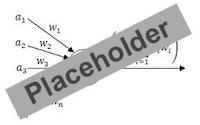
\includegraphics{images/neuron.png}
      		\caption{Illustration of a neuron as graph.}
	\end{minipage}
	\hfill
	\begin{minipage}[c]{0.5\linewidth}
	\centering
	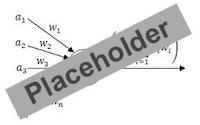
\includegraphics{images/neuron.png}
      		\caption{Illustration of a layer as graph.}
	\end{minipage}
\end{figure}

Logically one can use the output of a layer as input for another layer. Iteratively doing so will construct specific functions known as neural networks. In order to formalize this idea we denote the following definition. \\

\pagebreak
\begin{definition} \label{def:network}
Let $l \in \N$ and $d_0, \dots, d_l \in \N$. A neural network is defined as a function
\[ f : \R^{d_0} \to \R^{d_l} : x \mapsto f_l \circ f_{l-1} \circ \cdots \circ f_1 (x),\]
where each $f_i$ for $i=1, \dots, l$ is a layer with input dimension $d_{i-1}$ and output dimension $d_i$. Networks with a certain level of complexity, say $l>2$, are referred to as deep neural networks.
\end{definition}

Just like neurons and layers, neural networks can also be visualized as graphs.

\begin{figure}[!h]
\centering
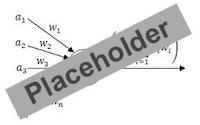
\includegraphics{images/neuron.png}
\caption{Illustration of a neural network as graph.}
\label{fig:neuron}
\end{figure}  

Neural networks find massive adoption in machine learning as they can model arbitrary complex functions. For example one could envision functions that predict the weather at a specific place and time or functions that determine if an image contains a cat or a dog. Clearly there is no simple mathematical formula to describe such problems. \\

A common practice to learn those functions is, to fix the number of layers, the number of neurons per layer as well as the activation functions, to choose some initial weights and then iteratively adjust the weights in order to approximate the unknown target function. This approach requires some mapping between a neural network and its weights. In the notion of definition \ref{def:network} one can determine the total number of weights in $f$ as
\[ n = \sum_{i=0}^{l-1} (d_i + 1) \cdot d_{i+1}. \]
Denoting these weights as a parameter vector $w \in \R^n$ enables us to define a function
\[ \tilde{f} : \R^d \times \R^n \to \R^p : (x,w) \mapsto \tilde{f}(x,w), \]
such that for fixed $w_1, w_2 \in \R^n$ the functions $\tilde{f}(x,w_1)$ and $\tilde{f}(x,w_2)$ are neural networks matching in their number of layers, number of neurons as well as activation functions and differing only in their choice of weights. One calls $\tilde{f}(x,w_1)$ and $\tilde{f}(x,w_2)$ realizations of the neural network architecture $\tilde{f}$. \\

In the following, the terms neural network and neural network architecture will be used synonymously if the meaning is clear by the context. Unless otherwise specified, $d \in \N$ will denote the dimension of the input space, $p \in \N$ will denote the dimension of the output space and $n \in \N$ will denote the number of adjustable weights.

\subsection{Training}\label{sec:Training}

Training a neural network refers to finding the optimal weights, given a fixed neural network architecture $\tilde{f} : \R^d \times \R^n \to \R^p$. In other words, finding a function $f \in \tilde{\F}$, where
\[ \tilde{\F} = \Big \{ f : \R^d \to \R^p : x \mapsto \tilde{f}(x,w) \mid w \in \R^n \Big \} \]
denotes the set of all neural networks with given architecture. In order to define a sense of optimality, we need a mechanism measuring the quality of network outputs. This is done by a loss function
\[ \L : \R^p \times \R^p \to \R : \big ( f(x,w),y \big ) \mapsto \L \big ( f(x,w),y \big ) ,\]
that should be chosen in such a way, that for some input $x \in \R^d$ with target output $y \in \R^p$ it associates some cost with the error between the prediction $f(x,w)$ and the true label $y$. \\

Under the assumption, that in reality there exists a probability distribution $\D$ on $\R^d \times \R^p$, describing the correlation between inputs $x \in \R^d$ and target values $y \in \R^p$, we call a weight vector $w_* \in \R^n$ to be optimal, if
\[ \forall w \in \R^n : R(w_*) \leq R(w), \]
where $R(w)$ denotes the so called risk or generalization error 
\[ R : \R^n \to \R : w \mapsto \E_{(x,y) \sim \D } \Big [ \L \big (f(x,w),y \big ) \Big ]. \]

For later use we will denote the marginal distribution of the inputs as $\D_x$. At this point it should be noted, that in general the underlying probability distribution $\D$ is unknown. Hence we can not evaluate the expectation in previous expression. \\

For this reason, the training of neural networks requires labeled training data
\[ \Big \{ (x_i,y_i) \in \R^d \times \R^p \mid i=1, \dots, m \Big \} \]
for some $m \in \N$. Instead of working with the generalization error, the training data enables us to minimize the empirical error function
 \[ E : \R^n \to \R : w \mapsto \frac{1}{m} \sum_{i=1}^{m} \L \big ( f(x_i,w),y_i \big) + \lambda \| w \|^2, \]
where $\lambda \in \R$ is some regularization parameter used to control the complexity of $w$. \\
 
Intuitively minimization of the empirical error should lead to a minimization of the generalization error as well. Currently, a lot of research is being done on how these measures relate to each other. Nevertheless this thesis will focus on how to minimize the empirical error given labeled training data. \\

The problem of finding some weight vector $w$ that minimizes the empirical error function is usually hard to solve as the error may have highly nonlinear dependencies on the weights. This is why in practice one often aims to compare several local minima and to settle for one that is sufficient enough, regardless of whether it is a global minimum or not.

\begin{definition}
Let $f: \R^n \to \R$ be differentiable. The gradient of $f$ is defined as
\[ \nabla f : \R^n \to \R^n : x = (x_1, \dots, x_n) \mapsto \bigg [ \frac{\partial}{\partial x_1} f(x), \cdots, \frac{\partial}{\partial x_n} f(x) \bigg ]^T. \]
\end{definition}

Due to the complexity of the error function, in general there is no easy way to find an analytical solution to the problem $\nabla E(w) = 0$. Hence most of the techniques for error minimization are based on iterative approximation. One popular method is gradient descent.

\begin{algorithm}
\caption{Gradient Descent} \ \\
Let $f: \R^n \to \R$ be differentiable. Gradient descent proceeds as follows: \\

1) Initialize $k=0$, choose $\epsilon \geq 0 \in \R$ and pick some random $x_0 \in \R^n$. \\

2) \textbf{while} $ \big \| \nabla f(x_k) \big \|_2 > \epsilon $ \textbf{do}:\\

\quad 3) Choose a step size $\alpha_k > 0 \in \R$. \\

\quad 4) Set $x_{k+1} = x_k - \alpha_k \cdot \nabla f(x_k)$ and $k = k+1$. \\

5) \textbf{end while} \\
\end {algorithm}

We will see, that in the case where $f$ is bounded from below and $\nabla f$ is Lipschitz continuous, we can guarantee the  converges of gradient descent to a stationary point.

\begin{definition}
Let $(\X,d_{\X})$ and $(\Y, d_{\Y})$ be two metric spaces. A function $f: \X \to \Y$ is called Lipschitz continuous, if there exists $L \geq 0$, such that
\[ \forall x,x' \in \X : d_{\Y} \big ( f(x) , f(x') \big ) \leq L \cdot d_{\X}(x,x'). \]
The smallest constant $L$, that suffices the previous condition is called Lipschitz constant of $f$.
\end{definition}

Casually speaking, the Lipschitz continuity of $\nabla f$ ensures that the gradient does not change heavily for two points that are close to each other.

\begin{definition}
Let $f: \R^n \to \R$. The set of stationary points of $f$ is defined as
\[ \big \{ x \in \R^n \mid \nabla f(x) = 0 \big \}. \]
\end{definition}

There a three kinds of stationary points: saddle points, local extrema and global extrema. We are especially interested in global minima as they provide the lowest possible error.

\begin{definition}
Let $\X$ be a subset of some real vector space and $f: \X \to \R$ be bounded from below. We call $x_* \in \X$ a global minimizer of $f$, if
\[ \forall x \in \X : f(x_*) \leq f(x). \]
\end{definition}

To prove convergence of the gradient descent algorithm for bounded $f$ with Lipschitz continuous gradient, we need an intermediate result, that is formulated in the following lemma.

\begin{lemma} \label{lem:descent}
Let $f: \R^n \to \R$ be differentiable, such that the gradient $\nabla f$ is Lipschitz continuous with Lipschitz constant $L>0$, then
\[ \forall x,y \in \R^n : f(y) \leq f(x) + \big \langle \nabla f(x) , y -x \big \rangle + \frac{L}{2} \big \| y - x \big \|_2^2. \]
\end{lemma}

\begin{proof}
Let $x,y \in \R^n$, define $z_{\lambda} := x + \lambda (y - x)$ for $\lambda \in \R$ and consider the function
\[ \phi : \R^n \mapsto \R : \lambda \mapsto f(z_{\lambda}) = f \big (x + \lambda (y-x) \big ). \]
Since $f$ is differentiable we can apply the chain rule to derive
\[ \phi' : \R^n \mapsto \R : \lambda \mapsto (y-x)^T \cdot \nabla f \big ( x + \lambda (y-x) \big ). \]
Integration over $\phi'$ from $\lambda = 0$ to $\lambda = 1$ yields
\[ \int_{0}^{1} \big \langle \nabla f(z_{\lambda}), y-x \big \rangle \ d\lambda = \int_{0}^{1} \phi'(\lambda) \ d \lambda = \phi(1) - \phi(0) = f(y) - f(x). \]
This equality can be rewritten as
\[ \begin{split} 
f(y) - f(x) 
&= \int_{0}^{1}\big \langle \nabla f(z_{\lambda}), y-x \big \rangle \ d\lambda \\\
&= \int_{0}^{1} \big \langle \nabla f(z_{\lambda}) - \nabla f(x) + \nabla f(x) , y-x\big \rangle \ d\lambda \\\
&= \big \langle \nabla f(x), y-x \big \rangle + \int_{0}^{1} \big \langle \nabla f(z_{\lambda}) - \nabla f(x), y-x \big \rangle \ d\lambda.
\end{split} \]
Using the Cauchy-Schwarz inequality we derive
\[ \begin{split}
\Big | \ f(y) - f(x) - \big \langle \nabla f(x), y-x \big \rangle \ \Big | 
&= \Big | \ \int_{0}^{1} \big \langle \nabla f(z_{\lambda}) - \nabla f(x), y-x \big \rangle \ d\lambda \ \Big | \\\
&\leq \int_{0}^{1} \Big | \ \big \langle \nabla f(z_{\lambda}) - \nabla f(x), y-x \big \rangle \ \Big | \ d\lambda \\\
&\leq \int_{0}^{1} \big \| \nabla f( z_{\lambda}) - \nabla f(x) \big \|_2 \cdot \big \| y-x \big \|_2 \ d\lambda.
\end{split} \]
Due to the Lipschitz continuty of $\nabla f$ we can use the upper bound 
\[ \big \| \nabla f( z_{\lambda}) - \nabla f(x) \big \|_2 \leq L \cdot \big \| z_{\lambda} - x \big \|_2 = L \cdot \big \| \lambda(y-x) \big \|_2 = L\lambda \cdot \big \| y-x \big \|_2 \]
for $\lambda \in [0,1]$, to conclude
\[ \Big | \ f(y) - f(x) - \big \langle \nabla f(x), y-x \big \rangle \ \Big | \leq \int_{0}^{1} L\lambda \cdot \big \| y-x \big \|_2^2 \ d\lambda = \frac{L}{2} \big \| y-x \big \|_2^2. \]
Rearranging the inequality finally yields
\[ f(y) \leq f(x) + \big \langle \nabla f(x) , y -x \big \rangle + \frac{L}{2} \big \| y - x \big \|_2^2. \]
This completes the proof, since $x,y$ were chosen arbitrary.
\end{proof}

\begin{theorem} \label{thm:descent}
Let $f: \R^n \to \R$ be differentiable with a global minimizer $x_* \in \R^n$, such that the gradient $\nabla f$ is Lipschitz continuous with Lipschitz constant $L>0$, then gradient descent with $\epsilon = 0$ and constant step size $\alpha_k = 1/L$ produces a sequence $(x_k)_{k \in \N_0} \in \R^n$, such that 
\[ \forall n \in \N : \min_{0 \leq k \leq n} \big \| \nabla f(x_k) \big \|_2^2 \leq \frac{2L \big ( f(x_0) - f(x_*) \big )}{n+1}. \]
\end{theorem}

\begin{proof}
Let $k \in \N$ be arbitrary. Since $f$ is differentiable with Lipschitz continuous gradient, we can apply lemma \ref{lem:descent} to derive
\[  f(x_{k+1}) \leq f(x_k) + \big \langle \nabla f(x_k) , x_{k+1} -x_k \big \rangle + \frac{L}{2} \big \| x_{k+1} - x_k \big \|_2^2. \]
By the definition of gradient descent, we can plug in $x_{k+1} - x_k = - 1/L \cdot \nabla f(x_k)$ to conclude
\[ \begin{split} 
f(x_{k+1}) 
&\leq f(x_k) + \big \langle \nabla f(x_k) , - \frac{1}{L} \nabla f(x_k) \big \rangle + \frac{L}{2} \big \| \frac{1}{L} \nabla f(x_k) \big \|_2^2 \\\
&= f(x_k) - \frac{1}{L} \big \| \nabla f(x_k) \big \|_2^2 + \frac{1}{2L} \big \| \nabla f(x_k) \big \|_2^2 \\\
&= f(x_k) - \frac{1}{2L} \big \| \nabla f(x_k) \big \|_2^2.
\end{split} \]
Hence the gradient descent algorithm with constant step size $\alpha_k = 1/L$ guarantees to make progress unless $\nabla f(x_k) \neq 0$. The previous expression is equivalent to
\[ \big \| \nabla f(x_k) \big \|_2^2 \leq 2L \big ( f(x_k) - f(x_{k+1}) \big ). \]
Summing up both sides from $k=0$ to some $n \in \N$ and taking the average results in
\[ \frac{1}{n+1} \sum_{k=0}^{n} \big \| \nabla f(x_k) \big \|_2^2 \leq \frac{2L}{n+1} \sum_{k=0}^{n} f(x_k) - f(x_{k+1}) = \frac{2L}{n+1} \big ( f(x_0) - f(x_{n+1}) \big ). \]
Using $f(x_*) \leq f(x_k)$ for every $k \in \N$, we conclude
\[ \min_{0 \leq k \leq n} \big \| \nabla f(x_k) \big \|_2^2 \leq \frac{1}{n+1} \sum_{k=0}^{n} \big \| \nabla f(x_k) \big \|_2^2 \leq \frac{2L}{n+1} \big ( f(x_0) - f(x_*) \big ). \]
This completes the proof, since $n$ was chosen arbitrary.
\end{proof}

Note that in practice it is inefficient to use a constant step size of $1/L$. Nevertheless it is useful for theoretical analysis to guarantee convergence. \\

Theorem \ref{thm:descent} states, that in the limit as $n \to \infty$, gradient descent converges to a stationary point $\hat{x} \in \R^n$ with $\nabla f(\hat{x}) = 0$. Since we have seen in the proof, that $f(x_k)$ is monotonically decreasing in $k$, gradient descent converges to the next stationary point in direction of descent, which is either a local minimum, a global minimum or a saddle point. \\

Next we will define a special class of functions having the nice property, that every stationary point is a global minimum and therefore gradient descent is an excellent tool for minimization.

\begin{definition}
Let $\X$ be a subset of some real vector space. $\X$ is said to be convex, if 
\[ \forall x, x' \in \X : \forall \lambda \in [0,1] : \lambda x + (1 - \lambda) x' \in \X. \]
\end{definition}

Casually speaking a set is convex if it contains the connection line between any two points in the set. Based on the notion of convex sets we can define convex functions.

\begin{definition}
Let $\X$ be a convex subset of some real vector space. A function $f: \X \to \R$ is said to be convex, if
\[ \forall x,x' \in \X : \forall \lambda \in [0,1] : f \big (\lambda x + (1-\lambda) x' \big ) \leq \lambda f(x) + (1- \lambda) f(x'). \]
\end{definition}

For later use we denote the following property of convex functions.

\begin{lemma} \label{lem:convexity}
Let $\X$ be a convex subset of some real vector space. For convex functions $f: \X \to \R$ and $g: \X \to \R$ the sum $f+g$ is convex as well.
\end{lemma}

\begin{proof}
Let $x,x' \in \X$ and $\lambda \in [0,1]$ be arbitrary, then
\[ \begin{split}
\big ( f+g \big )(\lambda x + (1-\lambda)x') 
&= f(\lambda x + (1-\lambda)x') + g(\lambda x + (1-\lambda)x') \\\
&\leq \lambda f(x) + (1- \lambda) f(x') + \lambda g(x) + (1- \lambda) g(x') \\\
&= \lambda \big ( f+g \big ) (x) + (1- \lambda) \big ( f+g \big )(x').
\end{split} \]
This shows the convexity of $f+g$.
\end{proof}

Functions that are convex and continuous differentiable have the nice property, that every stationary point is a global minimum.

\begin{lemma}
Let $f: \R^n \to \R$ be convex and continuous differentiable and $x \in \R^n$, then
\[ \nabla f(x) = 0 \ \Leftrightarrow \ \forall x' \in \R^n : f(x) \leq f(x').  \]
\end{lemma}

\begin{proof}
Let $x \in \R^n$ with $\nabla f(x) = 0$. For arbitrary $x' \in \R^n$ we define the function
\[ \phi : \R \to \R : \lambda \mapsto f(x) + \lambda \big ( f(x') - f(x) \big ) - f \big ( x + \lambda (x'-x) \big ), \]
which is continuous differentiable with derivative
\[ \phi' : \R \to \R : \lambda \mapsto f(x') - f(x) - \nabla f \big (x + \lambda(x'-x)\big )^T (x'-x). \]
Since $\phi$ is non-negative on the interval $[0,1]$ with $\phi(0) = 0$, we derive
\[ \phi'(0) = f(x') - f(x) - \nabla f(x)^T (x'-x) \geq 0. \]
Using $\nabla f(x) = 0$ we conclude
\[ \forall x' \in \R^n : f(x) \leq f(x'). \]
This completes the proof, since the backwards direction is trivial.
\end{proof}

Thus for lower bounded functions $f: \R^n \to \R$, that are convex and differentiable with Lipschitz continuous gradient $\nabla f$, we can guarantee the convergence of gradient descent to a global minimum due to theorem \ref{thm:descent}. Unfortunately this does not apply to the error function used for neural networks, but we will introduce a theoretical approach to prevent this problem in section \ref{sec:kernel}. \\

Recalling the definition of the empirical error function 
 \[ E : \R^n \to \R : w \mapsto \frac{1}{m} \sum_{i=1}^{m} \L \big ( f(x_i,w),y_i \big) + \lambda \| w \|^2, \]
we realize, that the computation effort needed to compute the gradients, depends on the number of training samples $m$. This is a severe problem for the gradient descent algorithm, since we have to train on a significant amount of data, to optimize the millions of parameters in deep neural networks. Thus, gradient descent on the empirical error function is computationally and time expensive, that even with heavy computing power it can be unfeasible to find good solutions. However, there exist several other optimization methods, that apply the same concept of minimizing a function along the slope of its surface. \\

Stochastic gradient descent is a variation of gradient descent, that aims to approximate the gradient of the objective function instead of computing the exact gradient. Doing so, stochastic gradient descent makes a trade-off between the accuracy and the time needed for gradient computation. The basic idea is to compute the gradient on a random fraction of the data set and use this as an estimation of the gradient on the whole data set. In each iteration $k \in \N$ one randomly draws a subset $I_k \subset \{ 1, \dots, m \}$ of size $| I_k | = b \in \N$ and uses
\[ \nabla E(w_k,I_k) := \frac{1}{b} \sum_{i \in I_k}^{}  \L \big ( f(x_i,w_k),y_i \big) + \lambda \| w_k \|^2 \]
as an approximation of $\nabla E(w_k)$. Although only a small amount of data is used for one single parameter update, during training most of the data will be used to fit the model due to the large number of iterative updates.
\pagebreak

\begin{algorithm}
\caption{Stochastic Gradient Descent (SGD)} \ \\
Let $E: \R^n \to \R$ be a differentiable empirical error function. SGD proceeds as follows: \\

1) Choose a batch size $b \in \N$, a number of epochs $K \in \N$ and pick some random $w_0 \in \R^n$. \\

2) \textbf{for} $k=1, \dots, \frac{Km}{b}$ \textbf{do}: \\

\quad 3) Draw a random subset $I_k \subset \{1, \dots, m \}$ of size $| I_k | = b$. \\

\quad 4) Choose a step size $\alpha_k > 0 \in \R$. \\

\quad 5) Set $w_{k+1} = w_k - \alpha_k \cdot \nabla E(w_k,I_k)$. \\

6) \textbf{end for} \\
\end{algorithm}

In here, an epoch describes one iteration on a number of samples that equals the size of the whole training dataset. A theoretical convergence analysis of stochastic gradient descent can be found in [?], but would exceed the scope of this theory. \\

Until now we have not discussed how to choose the step sizes $\alpha_k$. To simplify things, in practice one usually chooses a step size $\alpha > 0$, that stays constant across each iteration. Unfortunately a constant step size does not adapt to the specific local properties of the error surface at iteration $k \in \N$. One method that aims to improve the SGD algorithm by including past gradients for the current parameter update is the following.

\begin{algorithm}
\caption{Adaptive Moment Estimation (Adam)} \ \\
\textcolor{white}{$\Big |$}1: Requires differentiable empirical error function $E: \R^n \to \R$ and random $w_0 \in \R^n$.  \\
\textcolor{white}{$\Big |$}2: Requires constant step size $\alpha > 0 \in \R$, batch size $b \in \N$ and number of epochs $K \in \N$. \\
\textcolor{white}{$\Big |$}3: Requires momentum factors $\beta_1, \beta_2 \in [0,1)$ and a scalar $\epsilon > 0 \in \R$. \\
\textcolor{white}{$\Big |$}4: \textbf{for} $k=1, \dots, \frac{Km}{b}$ \textbf{do}: \\
\textcolor{white}{$\Big |$}5: \quad Draw a random subset $I_k \subset \{1, \dots, m \}$ of size $| I_k | = b$. \\
\textcolor{white}{$\Big |$}6: \quad Set $m_{k} = \beta_1 m_{k-1} + (1-\beta_1) \cdot \nabla E(w_k,I_k)$ and $\hat{m}_k = \frac{m_k}{1-\beta_1^k}$. \\
\textcolor{white}{$\Big |$}7: \quad Set $v_{k} = \beta_2 v_{k-1} + (s-\beta_2) \cdot \nabla E(w_k,I_k)^2$ and $\hat{v}_k = \frac{v_k}{1-\beta_2^k}$. \\
\textcolor{white}{$\Big |$}8: \quad Set $w_{k+1} = w_k - \alpha \cdot \frac{\hat{m}_k}{\sqrt{\hat{v}_k} + \epsilon}$. \\
\textcolor{white}{$\Big |$}9: \textbf{end for} \\
\end{algorithm}
\pagebreak

In here, all operations on vectors are performed element-wise. The scalar $\epsilon$ is used to prevent division by zero. The default setup proposed by the authors is to choose $\epsilon = 10^{-8}$, $\beta_1 = 0.9$ and $\beta_2 = 0.999$. We will always apply this default setting when working with Adam. \\

The three optimization methods introduced so far, all have in common, that they perform parameter updates on first order information only. This is due to the fact, that Hessian matrix computation for deep neural networks is infeasible due to the large number of parameters. However, later on we will see one can train neural networks in tiny subspaces, such that second order methods are applicable. One optimization algorithm, that includes second order information is the following.

\begin{algorithm}
\caption{Broyden-Fletcher-Goldfarb-Shanno (BFGS)} \ \\
\textcolor{white}{$\Big |$}1: Requires differentiable $f: \R^n \to \R$, random $x_0 \in \R^n$ and  $\epsilon \geq 0 \in \R$. \\
\textcolor{white}{$\Big |$}2: Initialize $k \leftarrow 0$, $B_0 \leftarrow I_n$. \\
\textcolor{white}{$\Big |$}3: \textbf{while} $ \| \nabla f(x_k) \|_2 > \epsilon $ \textbf{do}: \\
\textcolor{white}{$\Big |$}4: \quad Choose a step size $\alpha_k > 0 \in \R$. \\
\textcolor{white}{$\Big |$}5: \quad Update $x_{k+1} \leftarrow x_k - \alpha_k B_k \nabla f(x_{k})$. \\
\textcolor{white}{$\Big |$}6: \quad Let $s_k = x_{k+1} - x_{k}$ and $y_k = \nabla f(x_{k+1}) - \nabla f(x_{k})$. \\
\textcolor{white}{$\Big |$}7: \quad Let $\rho_k = (y_k^Ts_k)^{-1}$ and $V_k = I_n - \rho_k y_k s_k^T$. \\
\textcolor{white}{$\Big |$}8: \quad Update $B_{k+1} \leftarrow V_k^TB_{k}V_k + \rho_k s_k s_k^T$ and $k \leftarrow k+1$. \\
\textcolor{white}{$\Big |$}9: \textbf{end while}
\end{algorithm}

\pagebreak
\section{Kernel Gradient Descent} \label{sec:kernel}

The goal of this section is to introduce and investigate the neural tangent kernel, which was analyzed by Arthur Jacot, Franck Gabriel and Cl\'{e}ment Holger in \cite{NTK}. We start by motivating and giving the definition of functional derivatives and functional gradient descent. This leads to the definition of multi-dimensional kernels, which enable us to generalize the functional gradient descent to so called kernel gradient descent. Having this concept in mind, we will prove that the training of neural networks in the parameter space is linked to kernel gradient descent in the function space with respect to a special kernel, the neural tangent kernel.
\subsection{Functional Derivatives}

As seen in section \ref{sec:Training}, the training of neural networks via parameter optimization is usually accomplished by minimizing the empirical error
\[ E : \R^n \to \R : w \mapsto \frac{1}{m} \sum_{i=1}^{m} \L \big ( f(x_i,w),y_i \big) + \lambda \| w \|^2 \]
on labeled training data $(x_i,y_i) \in \R^d \times \R^p$ for $i=1, \dots, m$. Due to the non-convexity of the error function $E$ it is in general hard to find a global minimum. However, we will see, that this problem can be prevented by moving from the parameter space $\R^n$ to the function space
\[ \F:= \Big \{ f: \R^d \to \R^p \Big \}. \]
That is we are no longer optimizing the specific parameters of the unknown target function but rather the function itself. This requires the definition of a cost
\[ C: \F \to \R : f \mapsto \frac{1}{m} \sum_{i=1}^{m} \L \big ( f(x_i),y_i \big), \]
associating some cost to each element of the function space $\F$.  In this notion, we can write
\[ E = C \circ (w \mapsto f(x,w)). \]
In contrast to the weight optimization approach, the choice of a convex loss function $\L$ provides a convex cost $C$, since by lemma \ref{lem:convexity} the sum of convex functions is convex again. We will introduce the functional gradient descent method, that enables us to minimize $C$ in the function space $\F$ and is an analog to the gradient descent method in the parameter space $\R^n$. Since $C$ is convex in the function space, convergence to a global minimum will be guaranteed in contrast to the non-convex parameter optimization problem. \\

Note that this approach is great for theoretical analysis due to the advantage of convexity. In practice however, we are still in need of the explicit parameters $w \in \R^n$, that describe the objective function. Nevertheless we can use the analysis of functional gradient descent to get a better understanding of gradient descent in the function space. \\

Let us start with a slight reformulation of well known results from functional analysis, that will enable us to define the functional derivative of the cost $C$.

\begin{definition}
Given a real vector space $\mathcal{V}$, we define the dual space
\[ \mathcal{V}^* := \Big \{ \mu : \mathcal{V} \to \R \mid \mu \text{ linear and continuous} \Big \}. \]
The elements of $\mathcal{V}^*$ are referred to as linear functionals.
\end{definition}

Until now it is unclear how all of the elements in $\F^*$ arise. We will see that they can be constructed by the elements of $\F$. This procedure is based on the following lemma.

\begin{lemma}
Given a fixed probability distribution $\D_x$ on the input space $\R^d$, one can equip the function space $\F$ with the seminorm
\[ \| \cdot \|_{\D_x} : \F \to \R : f \mapsto \sqrt{\langle f , f \rangle_{\D_x}} \] 
in terms of the symmetric positive semidefinite bilinear form
\[ \langle \cdot,\cdot \rangle_{\D_x} : \F \times \F \to \R : (f,g) \mapsto \langle f,g \rangle_{\D_x} := \E_{x \sim \D_x} \Big [ f(x)^Tg(x) \Big ].\]
\end{lemma}

\begin{proof}
Let $f_1, f_2, f, g \in \F$ and $\lambda \in \R$. $\langle \cdot,\cdot \rangle_{\D_x}$ is indeed symmetric and bilinear since it suffices \\

(i) $\langle f_1 + f_2 , g \rangle_{\D_x} = \langle f_1 , g \rangle_{\D_x} + \langle f_2 , g \rangle_{\D_x}$:
\[ \begin{split}
\langle f_1 + f_2 , g \rangle_{\D_x}
&= \E_{x \sim \D_x} \Big [ \big ( f_1(x) + f_2(x) \big )^Tg(x) \Big ] \\\
&= \E_{x \sim \D_x} \Big [ f_1(x)^Tg(x) + f_2(x)^Tg(x) \Big ] \\\
&= \E_{x \sim \D_x} \Big [ f_1(x)^Tg(x) \Big ] + \E_{x \sim \D_x} \Big [ f_2(x)^Tg(x) \Big ] \\\
&= \langle f_1 , g \rangle_{\D_x} + \langle f_2 , g \rangle_{\D_x},
\end{split} \]

(ii) $\langle \lambda f , g \rangle_{\D_x} = \lambda \langle f, g \rangle_{\D_x}$:
\[ \langle \lambda f , g \rangle_{\D_x} = \E_{x \sim \D_x} \Big [ \lambda f(x)^Tg(x) \Big ] = \lambda \cdot \E_{x \sim \D_x} \Big [ f(x)^Tg(x) \Big ] = \lambda \langle f, g \rangle_{\D_x}, \]

(iii) $\langle f , g \rangle_{\D_x} = \langle g , f \rangle_{\D_x}$:
\[ \langle f , g \rangle_{\D_x} = \E_{x \sim \D_x} \Big [ f(x)^Tg(x) \Big ] = \E_{x \sim \D_x} \Big [ g(x)^Tf(x) \Big ] = \langle g , f \rangle_{\D_x}. \]

Furthermore $\langle \cdot,\cdot \rangle_{\D_x}$ is positive semidefinite, since for any $f \in \F$ it holds, that
\[ \langle f , f \rangle_{\D_x} =  \E_{x \sim \D_x} \Big [ f(x)^Tf(x) \Big ] = \E_{x \sim \D_x} \Big [ \sum_{i=1}^{d} f_i(x)^2 \Big ] \geq 0. \]

Thus $\| \cdot \|_{\D_x} = \sqrt{\langle \cdot , \cdot \rangle_{\D_x}}$ is a seminorm on the function space $\F$.
\end{proof}

\begin{lemma}
The seminorm $\| \cdot \|_{\D_x}$ induces the pseudometric
\[ d: \F \times \F \to \R_+ : (f,g) \mapsto \big \| f-g \big \|_{\D_x}, \]
such that $(\F,d)$ is a complete pseudometric space.
\end{lemma}

\begin{proof}
Let $f,g,h \in \F$. $d$ is indeed a pseudometric since it suffices \\

(i) $d(f,f) = 0$:
\[ d(f,f) = \big \| f - f \big \|_{\D_x} = 0, \]

(ii) $d(f,g) = d(g,f)$:
\[ d(f,g) = \big \| f - g \big \|_{\D_x} = \big \| g - f \big \|_{\D_x} = d(g,f), \]

(iii) $d(f,h) \le d(f,g) + d(g,h)$:
\[ \begin{split} 
d(f,h) &= \big \| f - h \big \|_{\D_x} \\\ &= \big \| f - g + g - h \big \|_{\D_x} \\\ &\le \big \| f - g  \big \|_{\D_x} + \big \| g - h \big \|_{\D_x} = d(f,g) + d(g,h). \end{split} \]

The completeness of $\F$ arises from the fact, that every Cauchy sequence in $\R$ converges.
\end{proof}

Based on the completeness of $\F$ one can introduce the concept of orthogonal projections.

\begin{lemma} \label{lem:projection}
Let $\A \subset \F$ be non-empty, closed and convex. For every $f \in \F$ there exists some $a^* \in \A$ such that 
\[ \big \| f - a^* \big \|_{\D_x}^2 = \inf_{a \in \A} \big \| f - a \big \|_{\D_x}^2. \]
Such an element $a^*$ is called orthogonal projection of $f$ on $\A$.
\end{lemma}

\begin{proof}
Let $f \in \F$. There exists a sequence $(a_n)_{n \in \N} \subset \A$ such that
\[ \lim_{n \to \infty} \big \| f - a_n \big \|_{\D_x}^2 = \inf_{a \in \A} \big \| f - a \big \|_{\D_x}^2 =: \delta. \]
For $n,m \in \N$ we can derive
\[ \begin{split}
\big \| a_n - a_m \big \|_{\D_x}^2 
&= \big \| (f-a_n) - (f-a_m) \big \|_{\D_x}^2 \\\
&= \big \| f - a_n \big \|_{\D_x}^2 + \big \| f - a_m \big \|_{\D_x}^2 - 2 \big \langle f-a_n, f-a_m \big \rangle_{\D_x}.
\end{split} \]
Furthermore we have
\[ \big \| (f-a_n) + (f-a_m) \big \|_{\D_x}^2 = \big \| f - a_n \big \|_{\D_x}^2 + \big \| f - a_m \big \|_{\D_x}^2 + 2 \big \langle f-a_n, f-a_m \big \rangle_{\D_x}. \]

Combining both expressions yields
\[ \begin{split}
\big \| a_n - a_m \big \|_{\D_x}^2 
&= 2 \big \| f - a_n \big \|_{\D_x}^2 + 2 \big \| f - a_m \big \|_{\D_x}^2 - \big \| (f-a_n) + (f-a_m) \big \|_{\D_x}^2 \\\
&= 2 \big \| f - a_n \big \|_{\D_x}^2 + 2 \big \| f - a_m \big \|_{\D_x}^2 - 4 \big \| f - \frac{1}{2}(a_n+a_m) \big \|_{\D_x}^2.
\end{split} \]

Since $\A$ is convex, $\frac{1}{2}(a_n + a_m) \in \A$, such that for arbitrary $\epsilon > 0$ there exists $N \in \N$ with 
\[ \big \| a_n - a_m \big \|_{\D_x}^2 \leq 2(\delta + \epsilon) + 2(\delta + \epsilon) - 4\delta = 4\epsilon \]
for any $n,m > N$. Thus $(a_n)_{n \in \N}$ is a Cauchy sequence. Since $\F$ is complete and $\A$ is closed, $(a_n)_{n \in \N}$ converges to some $a^* \in \A$ with $\big \| f - a^* \big \|_{\D_x}^2 = \delta$.
\end{proof}

Lemma \ref{lem:projection} is a weakening of the Hilbert projection theorem stating that, given a Hilbert space, it even exists a unique orthogonal projection. In our case we lose the uniqueness, beacuse $\F$ is only a pseudometric space and not a metric space. However this is just a side note, since the existence of an orthogonal projection suffices for the further theory.

\begin{corollary} \label{cor:projection}
Let $f \in \F$ and $\A \subset \F$ be a non-empty and closed subspace. For every $a \in \A$ it holds, that $\langle f - a^* , a \rangle_{\D_x} = 0$, where $a^* \in \A$ denotes an orthogonal projection of $f$ on $\A$.
\end{corollary}

\begin{proof}
Let $a \in \A$ and $\lambda \in \R$. Since $\A$ is a subspace we can infer $a^* + \lambda a \in \A$. Thus we derive
\[ \big \| (a^* + \lambda a) -f \big \|_{\D_x}^2 \geq \big \| a^* - f \big \|_{\D_x}^2 \]
by the minimality of $a^*$. Rearranging the inequality yields
\[ \big \| (a^* - f) + \lambda a \big \|_{\D_x} ^2 - \big \| a^* - f \big \|_{\D_x}^2 = 2 \big \langle a^* -f , \lambda a \big \rangle_{\D_x} + \big \| \lambda a \big \|_{\D_x}^2 \geq 0, \]
giving rise to the definition of the non-negative function
\[ \phi : \R \to \R : \lambda \mapsto 2 \lambda \big \langle a^* -f , a \big \rangle_{\D_x} + \lambda^2 \big \| a \big \|_{\D_x}^2. \]
Under the assumption that $\big \langle a^* - f , a \big \rangle_{\D_x} \neq 0$ and $\| a \|_{\D_x}^2 \neq 0$, we derive
\[ \phi \Big ( - \frac{ \big \langle a^* - f , a \big \rangle_{\D_x}}{\| a \|_{\D_x}^2} \Big ) = -2 \cdot \frac{ \big \langle a^* - f , a \big \rangle_{\D_x}^2}{ \| a \|_{\D_x}^2} + \frac{\big \langle a^* - f , a \big \rangle_{\D_x}^2}{ \| a \|_{\D_x}^2} = - \frac{ \big \langle a^* - f , a \big \rangle_{\D_x}^2}{ \| a \|_{\D_x}^2} < 0 \]
and under the assumption that $\big \langle a^* - f, a \big \rangle_{\D_x} \neq 0$ and $\| a \|_{\D_x}^2 = 0$, we derive
\[ \phi \Big ( -  \big \langle a^* - f , a \big \rangle_{\D_x} \Big ) = -2 \cdot \big \langle a^* - f , a \big \rangle_{\D_x}^2 < 0, \]
which is a contradiction to $\phi(\lambda) \geq 0$ for every $\lambda \in \R$. Thus $ \big \langle f - a^* , a \big \rangle_{\D_x} = 0$.
\end{proof}

Finally, the concept of orthogonal projections enables us to represent any functional $\mu \in \F^*$ based on a representer $d \in \F$.

\begin{lemma} \label{lem:riesz}
The map
\[ J: \F \to \F^* : d \mapsto \langle d, \cdot \rangle_{\D_x} \]
is linear and surjective.
\end{lemma}

\begin{proof}
The linearity follows directly from the linearity of $\langle \cdot, \cdot \rangle_{\D_x}$. To prove that $J$ is indeed surjective, we let $\mu \in \F^*$ and need to find some $d \in \F$ such that $\mu = J(d)$. \\

Case $\mu=0$: We can choose $d=0$, with $\mu = 0 = J(d)$. \\

Case $\mu \neq 0$: Due to the linearity of $\mu$ we can normalize and find some $e \in \F$ with $\mu[e] = 1$. Let $N:=\mu^{-1}(0)$ denote the kernel of $\mu$, which is non-empty, closed and convex since $\mu$ is linear and continuous. Thus by Lemma \ref{lem:projection} there exists some $p_e \in N$, such that $p_e$ is an orthogonal projection of $e$ on $N$. Define $f := e - p_e$, then $f \notin N$ since
\[ \mu[f] = \mu[e] - \mu[p_e] = \mu[e] = 1. \]
Based on the linearity of $\mu$, we can derive for arbitrary $g \in \F$, that
\[ \mu \big [g- \mu[g]f \big] = \mu[g] - \mu[g] \mu[f] = \mu[g] - \mu[g] \cdot 1 = 0 , \]
which implies $h := g - \mu[g]f \in N$. Thus $\langle f , h \rangle_{\D_x} = 0$ by corollary \ref{cor:projection} and we conclude
\[ \langle f, g \rangle_{\D_x} = \langle f , h \rangle_{\D_x} + \langle f , \mu[g]f \rangle_{\D_x} = 0 + \mu[g] \cdot \langle f , f \rangle_{\D_x} = \mu[g] \cdot \| f \|_{\D_x}^2. \]
Now we can assume that $\| f \|_{\D_x}^2 \neq 0$. Otherwise we would have $\langle f, g \rangle_{\D_x} = 0$ for every $g \in \F$ and therefore $f = 0$ which is a contradiction to $f \notin N$. Rearranging terms results in
\[ \mu[g] = \big \langle f / \| f \|_{\D_x}^2 , g \big \rangle_{\D_x} = J \big (f / \| f \|_{\D_x}^2 \big)[g]. \]
Hence we have found $d = f / \| f \|_{\D_x}^2$ with $\mu = J(d)$. This shows surjectivity.
\end{proof}

Thus for each functional $\mu \in \F^*$ there exists $d \in \F$ such that $\mu = \langle d, \cdot \rangle_{\D_x}$. In other words
\[ \F^* = \Big \{ \mu : \F \to \R : f \mapsto \langle d,f \rangle _{\D_x} \mid d \in \F \Big \}. \]

Lemma \ref{lem:riesz} is a weakening of the Riesz representation theorem stating that any Hilbert space $\H$ is isometric and isomorphic to its dual space $\H^*$ via the map $J:\H \to \H^* : x \mapsto \langle x , \cdot \rangle_\H$. \\

Since $\langle \cdot , \cdot \rangle_{\D_x}$ is only positive semidefinite and not positive definite we lose the property of $J$ being isometric and therefore injective. Again, this is just a side note, since surjectivity will be sufficient enough for the further theory. Note that, based on the definition of $\D_x$, $J$ maps two elements of $\F$ to the same functional, if and only if they are equal on the data.  \\

The representation theorem has great importance for the functional gradient descent method. Another crucial ingredient is the definition of functional derivatives and functional gradient.

\begin{definition} \label{def:derivative}
Let $\phi, f_0 \in \F$. A functional $\mu: \F \to \R$ is said to be differentiable at the point $f_0$ in direction $\phi$, if
\[ \int \frac{\partial\mu}{\partial f_0(x)}(x)\phi(x) \ dx = \lim_{\epsilon \to 0} \frac{\mu[f_0 + \epsilon \phi] - \mu[f_0]}{\epsilon} \]
exists. The functional gradient of $\mu$ at $f_0$ is defined as 
\[ \nabla \mu |_{f_0} : \R^d \to \R^p : x \mapsto \frac{\partial \mu}{\partial f_0(x)}(x). \]
 If the limit exists for every $\phi \in \F$ we define the functional derivative of $\mu$ at $f_0$ as
\[ \partial_{f} \mu |_{f_0} : \F \to \R : \phi \mapsto \frac{\partial}{\partial \epsilon} \Big [ \mu[f_0+\epsilon \phi] \Big ]_{\epsilon=0}. \]
\end{definition}

Based on these definitions, we can iteratively minimize functionals $\mu: \F \to \R$ in a similar manner to the gradient descent method.

\begin{algorithm}
\textbf{------------------------------------------------------------------------------------------------------} \\
Let $\mu: \F \to \R$ be differentiable. Functional gradient descent proceeds as follows: \\

1) Initialize $k=0$, choose $\epsilon \geq 0 \in \R$ and pick some random $f_0 \in \F$. \\

2) WHILE $ \big \| \nabla \mu |_{f_k} \big \|_{\D_x} > \epsilon $ DO:\\

\quad 3) Choose a step size $\alpha_k > 0 \in \R$. \\

\quad 4) Set $f_{k+1} = f_k - \alpha_k \cdot \nabla \mu |_{f_k}$ and $k = k+1$. \\
\textbf{------------------------------------------------------------------------------------------------------} 
\end {algorithm}

With a slight change in notation, the same argumentation that was used for convergence of gradient descent on functions, can be applied to the functional gradient descent method. \\

Until now we have a theoretical understanding of functional gradient descent in the function space $\F$. However there is not yet a connection to gradient descent in the parameter space. In theory, functional gradient descent is an excellent tool to guarantee convergence but in practice we need the explicit parameter vector $w \in \R^n$ to represent the optimal function due to functional gradient descent. This relationship between functional gradient descent and parameter gradient descent can be established by so called kernel gradient descent. 

\subsection{Kernel Gradient}

We start by recalling the basic definition of one-dimensional kernels.

\begin{definition}
Let $X$ be an arbitrary set. A one-dimensional kernel over $X$ is a map 
\[ K: X \times X \to \R : (x,x') \mapsto K(x,x').\]
A kernel $K$ is said to be positive definite symmetric if for any $m \in \N$ and $x \in X^m$, the matrix with entries $M_{i,j} = K(x_i,x_j)$ for $i,j = 1, \dots, m$ is symmetric and positive semidefinite.
\end{definition}

This thesis will work with kernels over the input space $\R^d$, not only with one-dimensional but with multi-dimensional kernels, which motivates the following definition.

\begin{definition}
A multi-dimensional kernel over $\R^d$ is a function
\[ K: \R^d \times \R^d \to \R^{p \times p} : (x,x') \mapsto K(x,x'), \]
such that $K(x,x') = K(x',x)^T$ for any $x,x' \in \R^d$.
\end{definition}

Based on the marginal distribution $\D_x$, kernels induce symmetric bilinear forms.

\begin{lemma} \label{lem:form}
A kernel $K: \R^d \times \R^d \to \R^{p \times p}$ induces the symmetric bilinear form
\[ \langle \cdot, \cdot \rangle_K : \F \times \F \to \R : (f,g) \mapsto \langle f , g \rangle _K := \E_{x,x' \sim \D_x} \Big [ f(x)^T K(x,x') g(x') \Big ], \]
where $x, x' \in \R^d$ are drawn independently according to $\D_x$. 
\end{lemma}

\begin{proof}
Let $f_1, f_2, f, g \in \F$ and $\lambda \in \R$. $\langle \cdot,\cdot \rangle_{K}$ is indeed symmetric and bilinear since it suffices \\

(i) $\langle f_1 + f_2 , g \rangle_{K} = \langle f_1 , g \rangle_{K} + \langle f_2 , g \rangle_{K}$:
\[ \begin{split}
\langle f_1 + f_2 , g \rangle_{K}
&= \E_{x,x' \sim \D_x} \Big [ \big ( f_1(x) + f_2(x) \big )^TK(x,x')g(x') \Big ] \\\
&= \E_{x,x' \sim \D_x} \Big [ f_1(x)^TK(x,x')g(x') + f_2(x)^TK(x,x')g(x') \Big ] \\\
&= \E_{x,x' \sim \D_x} \Big [ f_1(x)^TK(x,x')g(x') \Big ] + \E_{x,x' \sim \D_x} \Big [ f_2(x)^TK(x,x')g(x') \Big ] \\\
&= \langle f_1 , g \rangle_{K} + \langle f_2 , g \rangle_{K},
\end{split} \]

(ii) $\langle \lambda f , g \rangle_{K} = \lambda \langle f, g \rangle_{K}$:
\[ \begin{split} 
\langle \lambda f , g \rangle_{K} 
&= \E_{x,x' \sim \D_x} \Big [ \lambda f(x)^TK(x,x')g(x') \Big ] \\\
&= \lambda \cdot \E_{x,x' \sim \D_x} \Big [ f(x)^TK(x,x')g(x') \Big ] = \lambda \langle f, g \rangle_{K}, 
\end{split} \]

(iii) $\langle f , g \rangle_{K} = \langle g , f \rangle_{K}$:
\[ \begin{split} \langle f , g \rangle_{K} 
&= \E_{x,x' \sim \D_x} \Big [ f(x)^TK(x,x')g(x') \Big ] \\\
&= \E_{x,x' \sim \D_x} \Big [ f(x)^TK(x',x)^Tg(x') \Big ] \\\
&= \E_{x,x' \sim \D_x} \Big [ g(x')^TK(x',x)f(x) \Big ] = \langle g , f \rangle_{K}.
\end{split} \]

In contrast to $\langle \cdot , \cdot \rangle_{\D_x}$, the bilinear map $\langle \cdot , \cdot \rangle_{K}$ is not necessarily positive semidefinite.
\end{proof}

Using these bilinear forms, one can generalize the definition of positive definite kernels.

\begin{definition}
A kernel $K: \R^d \times \R^d \to \R^{p \times p}$ is called positive definite with respect to the seminorm $\| \cdot \| _{\D_x}$ if for every $f \in \F$ it holds, that $\| f \|_{\D_x} > 0$ implies $\langle f, f \rangle_K > 0$.
\end{definition}

We can use positive definite kernels to equip $\F$ with another seminorm.

\begin{lemma}
Given a kernel $K: \R^d \times \R^d \to \R^{p \times p}$, that is positive definite with respect to the seminorm $\| \cdot \|_{\D_x}$ we can use the bilinear form $\langle \cdot, \cdot \rangle_K$ to define another seminorm
\[ \| \cdot \|_K: \F \to \R : f \mapsto \sqrt{\langle \cdot, \cdot \rangle_K}.  \]
\end{lemma}

\begin{proof}
Since $\langle \cdot, \cdot \rangle_K$ is symmetric by lemma \ref{lem:form} it remains to show that $\langle \cdot, \cdot \rangle_K$ is positive semidefinite. For this we let $f \in \F$ be arbitrary and investigate the following cases. \\

Case $\| f \|_{\D_x} > 0$: Since $K$ is positive definite with respect to $\| \cdot \| _{\D_x}$, we derive $\langle f, f \rangle_K > 0$. \\

Case $\| f \|_{\D_x} = 0$: By the definition of $\langle \cdot , \cdot \rangle_{\D_x}$, we derive
\[ \big \| f \big \|_{\D_x}^2 = \langle f , f \rangle_{\D_x} = \E_{x \sim \D_x} \Big [ f(x)^Tf(x) \Big ] = \E_{x \sim \D_x} \Big [ \sum_{i=1}^{d} f_i(x)^2 \Big ] = 0. \]
Thus for every $x \sim \D_x$ it holds that $f(x) = 0$. Therefore we conclude
\[ \langle f , f \rangle_{K} = \E_{x,x' \sim \D_x} \Big [ f(x)^TK(x,x')f(x') \Big ] = 0. \]
In total we have shown that $\langle f, f \rangle_K > 0$ for every $f \in \F$, such that $\| \cdot \|_K$ is a seminorm.
\end{proof}

This concludes the necessary knowledge on kernels. Next we will introduce the kernel gradient of a functional, which is based on the partial application of kernels.

\begin{definition}
Let $K: \R^d \times \R^d \to \R^{p \times p}$ be a kernel. For $j=1, \dots, p$ one defines the partial application of $K$ as the function
\[ K_{\cdot,j} : \R^d \times \R^d \to \R^p : (x,x') \mapsto K(x,x')_{\cdot,j}, \]
where $K(x,x')_{\cdot,j}$ denotes the $j$-th column of the $p \times p $ matrix $K(x,x')$.
\end{definition}

Fixing one argument of $K_{\cdot,j}$ results in a function in $\F$. This enables the following definition.

\begin{definition}
Given a kernel $K: \R^d \times \R^d \to \R^{p \times p}$, we define the map
\[ \Phi_K : \F^* \to \F : \mu \mapsto f_{\mu}, \]
mapping a dual element $\mu \in \F$ to the function
\[ f_{\mu} : \R^d \to \R^p : x \mapsto \begin{bmatrix} \mu [K_{\cdot,1}(\cdot,x) ] \\ \vdots \\ \mu [ K_{\cdot,p}(\cdot,x)] \end{bmatrix}. \]
\end{definition}

Based on the definition of $\Phi_K$ we can define the kernel gradient of a functional.

\begin{definition}
Let $f_0 \in \F$, $\mu : \F \to \R$ be a differentiable functional with $\partial_f\mu|_{f_0} \in \F^*$ and $K$ be a kernel. The kernel gradient of $\mu$ at $f_0$ with respect to $K$ is defined as
\[ \nabla_K\mu|_{f_0}: \R^d \to \R^p : x \mapsto \Phi_K \Big ( \partial_f\mu|_{f_0} \Big )(x). \]
\end{definition}

Using this definition, we can formulate the kernel gradient descent method.

\begin{algorithm}
\textbf{------------------------------------------------------------------------------------------------------} \\
Let $K$ be a kernel and $\mu: \F \to \R$ be a differentiable functional with $\partial_f\mu|_{f_0} \in \F^*$. Kernel gradient descent with respect to the kernel $K$ proceeds as follows: \\

1) Initialize $k=0$, choose $\epsilon \geq 0 \in \R$ and pick some random $f_0 \in \F$. \\

2) WHILE $ \big \| \nabla_K \mu|_{f_k} \big \|_{\D_x} > \epsilon $ DO:\\

\quad 3) Choose a step size $\alpha_k > 0 \in \R$. \\

\quad 4) Set $f_{k+1} = f_k - \alpha_k \cdot \nabla_K \mu|_{f_k}$ and $k = k+1$. \\
\textbf{------------------------------------------------------------------------------------------------------}
\end {algorithm}

In the following, we will apply kernel gradient descent to minimize the cost $C$. During this we are especially interested in the evolution of the parameters defining the sequence $(f_k)_{k \in \N_0}$. \\

With the choice of a differentiable loss function, the cost functional $C : \F \to \R$ is differentiable as well, such that the functional derivative $\partial_{f} C |_{f_0}$ is well-defined for every $f_0 \in \F$. \\

In the following we will make the restriction, that the marginal distribution $\D_x$ on the input space $\R^d$ is given by the empirical distribution on a finite subset of $\R^d$. This means there exist $m \in \N$ and $x_1, \dots, x_m \in \R^d$ such that 
\[ \D_x = \frac{1}{m} \sum_{i=1}^{m} \delta_{x_i}, \]
where $\delta_{x_i}$ denotes the Dirac measure in $x_i$ for $i=1,\dots,m$. Under this assumption, the cost $C$ depends only on the values of $f$ at a finite dataset. Thus we conclude, that $\partial_{f} C |_{f_0}$ is linear and continuous and therefore $\partial_{f} C |_{f_0} \in \F^*$ for every $f_0 \in \F$. Hence by Lemma \ref{lem:riesz} there exists a representer $d|_{f_0} \in \F$, such that the functional derivative of $C$ can be written as
\[ \partial_{f} C |_{f_0} = \big \langle d|_{f_0}, \cdot \big \rangle_{\D_x}. \]

Next we will use this restriction on the distribution $\D_x$, to simplify the notation of $\Phi_K$.

\begin{lemma} \label{lem:phi}
Let $\mu = \langle d, \cdot \rangle_{\D_x} \in \F^*$ and $K: \R^d \times \R^d \to \R^{p \times p}$ be a kernel, then
\[ \Phi_K(\mu) = \frac{1}{m}\sum_{i=1}^{m} K(\cdot,x_i)d(x_i), \]
where $x_1, \dots, x_m \in \R^d$ denotes the finite support of the empiricial distribution $\D_x$.
\end{lemma}

\begin{proof}
Let $x \in \R^d$ be arbitrary. By the definition of $\Phi_K$ we have
\[ \Phi_K \big ( \mu \big )(x) = \Phi_K \Big ( \langle d, \cdot \rangle_{\D_x} \Big )(x) = \begin{bmatrix} \mu [K_{\cdot,1}(\cdot,x) ] \\ \vdots \\ \mu [ K_{\cdot,p}(\cdot,x)] \end{bmatrix} = \begin{bmatrix} \big \langle d, K_{\cdot,1}(\cdot,x) \big \rangle_{\D_x} \\ \vdots \\ \big \langle d, K_{\cdot,p}(\cdot,x) \big \rangle_{\D_x} \end{bmatrix}. \]
Recalling the definition of $\langle \cdot , \cdot \rangle_{\D_x}$, it holds that
\[ \big \langle d, K_{\cdot,j}(\cdot,x) \big \rangle_{\D_x} = \E_{x' \sim \D_x} \Big [ d(x')^TK_{\cdot,j}(x',x) \Big ] \]
for $j = 1, \dots, p$. Thus we derive
\[ \Phi_K \big ( \mu \big )(x) = \begin{bmatrix} \big \langle d, K_{\cdot,1}(\cdot,x) \big \rangle_{\D_x} \\ \vdots \\ \big \langle d, K_{\cdot,p}(\cdot,x) \big \rangle_{\D_x} \end{bmatrix} = \E_{x' \sim \D_x} \begin{bmatrix} d(x')^TK_{\cdot,1}(x',x) \\ \vdots \\ d(x')^TK_{\cdot,p}(x',x) \end{bmatrix} = \E_{x' \sim \D_x} \Big [ d(x')^T K(x',x) \Big ]^T. \]
With $K(x',x)^T = K(x,x')$ for every $x,x' \in \R^d$ by definition, we conclude
\[ \Phi_K \big ( \mu \big )(x) = \E_{x' \sim \D_x} \Big [ d(x')^T K(x',x) \Big ]^T = \E_{x' \sim \D_x} \Big [ K(x',x)^Td(x') \Big ] = \E_{x' \sim \D_x} \Big [ K(x,x')d(x') \Big ]. \]
The last step consists of using the assumption, that $\D_x$ is the empirical distribution on a finite dataset $x_1, \dots, x_m \in \R^d$. This enables us to derive
\[ \Phi_K \big ( \mu \big )(x) = \E_{x' \sim \D_x} \Big [ K(x,x')d(x') \Big ] = \frac{1}{m}\sum_{i=1}^{m} K(x,x_i)d(x_i). \]
This proves the statement of the lemma.
\end{proof}

By lemma \ref{lem:phi} we can write the kernel gradient of $C$ at $f_0$ with respect to some kernel $K$ as
\[ \nabla_KC|_{f_0}(x) = \Phi_K \Big ( \big \langle d|_{f_0} , \cdot \big \rangle_{\D_x} \Big )(x) = \frac{1}{m} \sum_{i=1}^{m} K(x,x_i)d|_{f_0}(x_i). \]

Due to the definition of the kernel, $\nabla_KC|_{f_0}$ has the advantage of being well-defined on the whole input space $\R^d$, where as the partial derivative $\partial_fC|_{f_0} =\langle d|_{f_0}, \cdot \rangle_{\D_x}$ is based on the bilinear form $\langle \cdot, \cdot \rangle_{\D_x}$ and therefore only defined on the finite dataset.

\begin{definition}
Let $K$ be a kernel. A time dependent function $f : \R \to \F$ is said to follow the kernel gradient descent on $C$ with respect to K if it satisfies the differential equation
\[ \partial_tf(t) = - \nabla_KC|_{f(t)}. \]
\end{definition}

We can think of such a function as a continuous extension to the sequence produced by kernel gradient descent on $C$, which can be used to investigate the change in $C$.

\begin{lemma}
Let $K$ be a positive definite kernel with respect to $\| \cdot \|_{\D_x}$ and $f: \R \to \F$ be a time dependent function, that follows the kernel gradient descent on $C$ with respect to $K$, then the evolution of $C \circ f$ during kernel gradient descent is expressed by
\[ \partial_tC|_{f(t)} = - \big \| d|_{f(t)} \big \|_{K}^2, \]
where $d|_{f(t)} \in \F$ denotes the representer of $\partial_f C|_{f(t)} = \big \langle d|_{f(t)}, \cdot \big \rangle_{\D_x} \in \F^*$ for $t \in \R$.
\end{lemma}

\begin{proof}
Using the notation $C|_{f(t)} = C \big [f(t) \big ]$, we derive
\[ \partial_tC|_{f(t)} = \partial_f C|_{f(t)} \big [ \partial_t f(t) \big ] = \big \langle d|_{f(t)}, \cdot \big \rangle_{\D_x} \big [ \partial_t f(t) \big ] = \big \langle d|_{f(t)}, \partial_t f(t) \big \rangle_{\D_x}. \]
Since $f$ follows the kernel gradient descent on $C$ with respect to $K$ this can be rewritten as
\[ \partial_tC|_{f(t)} = \big \langle d|_{f(t)}, \partial_t f(t) \big \rangle_{\D_x} = \big \langle d|_{f(t)}, - \nabla_K C|_{f(t)} \big \rangle_{\D_x}. \]
Recalling the definition of $\nabla_K C|_{f(t)}$, which was given by
\[ \nabla_KC|_{f(t)} = \frac{1}{m} \sum_{i=1}^{m} K(\cdot,x_i)d|_{f(t)}(x_i), \]
we derive by the linearity of $\langle \cdot, \cdot \rangle_{\D_x}$, that
\[ \begin{split} 
\big \langle d|_{f(t)}, - \nabla_K C|_{f(t)} \big \rangle_{\D_x} 
&= - \frac{1}{m} \sum_{i=1}^{m} \big \langle d|_{f(t)}, K(\cdot,x_i)d|_{f(t)}(x_i) \big \rangle_{\D_x} \\\
&= - \frac{1}{m} \sum_{i=1}^{m} \E_{x \sim \D_x} \Big [ d|_{f(t)}(x)^TK(x,x_i)d|_{f(t)}(x_i) \Big ] \\\
&= - \E_{x' \sim \D_x} \E_{x \sim \D_x} \Big [ d|_{f(t)}(x)^TK(x,x')d|_{f(t)}(x') \Big ]
= - \big \langle d|_{f(t)}, d|_{f(t)} \big \rangle_{K}.
\end{split} \]
Finally we conclude, that
\[ \partial_tC|_{f(t)} = \big \langle d|_{f(t)}, - \nabla_K C|_{f(t)} \big \rangle_{\D_x} = - \big \langle d|_{f(t)}, d|_{f(t)} \big \rangle_{K} = - \big \| d|_{f(t)} \big \|_{K}^2. \]
This completes the proof.
\end{proof}

The lemma guarantees the convergence of $C$ to a critical point, as $\partial_tC|_{f(t)} \leq 0$. In the case where $C$ is convex and bounded from below, this implies the convergence of $f(t)$ to a global minimum $f^* \in \F$ for $t \to \infty$.

\subsection{Kernel Approximation} \label{sec:approximation}

This subsection illustrates the relationship between gradient descent in the parameter space and kernel gradient descent in the function space under the assumption, that the objective function depends linear on its parameters. The example given in here, will be generalized later on, leading to the definition of the neural tangent kernel. \\

To start things off, we let $\D_{\F}$ be any probability distribution on the function space $\F$ and construct a kernel $K$, such that for $x,x' \in \R^d$ the image $K(x,x')$ is a $p \times p$ matrix defined by
\[ K_{i,j}(x,x') := \E_{f \sim \D_{\F}} \Big [ f_i(x) \cdot f_j(x) \Big ], \quad i,j=1,\dots,p. \]
We will see, that this kernel can be approximated by random functions. For this we choose some $n \in \N$ and draw $n$ random functions $f^{(k)} : \R^d \to \R^p$ for $k=1,\dots,n$ independently from the distribution $\D_{\F}$. Using these, we can define the linear map
\[ F^\textit{lin}: \R^n \to \F : w \mapsto f_w := \frac{1}{\sqrt{n}} \sum_{k=1}^{n}w_kf^{(k)}, \]
whose partial derivatives for $k=1,\dots,n$ are given by
\[ \partial_{w_{k}}F^\textit{lin} : \R^n \to \F: w \mapsto \frac{1}{\sqrt{n}}f^{(k)}. \]

Based on $F^\textit{lin}$ we can define another kernel, that will be used for the approximation of $K$.

\begin{definition}
For $x \in \R^p$ we define the symmetric matrix $x \otimes x := M \in \R^{p \times p}$, where
\[ M_{i,j} := x_i \cdot x_j, \quad  i,j=1,\dots,p. \]
\end{definition}

\begin{definition}
Given $n$ random functions $f^{(k)} : \R^d \to \R^p$ for $k=1,\dots,n$ drawn i.i.d. according to some distribution $\D_{\F}$ on the function space $\F$, the tangent kernel is defined as
\[ \tilde{K} := \sum_{k=1}^{n} \partial_{w_k} F^\textit{lin}(w) \otimes \partial_{w_k} F^\textit{lin}(w) = \frac{1}{n} \sum_{k=1}^{n} f^{(k)} \otimes f^{(k)}. \]
\end{definition}

In other words, $\tilde{K}$ maps a tuple $(x,x') \in \R^d \times \R^d$ to the matrix $\tilde{K} \in \R^{p \times p}$ with entries 
\[ \tilde{K}_{i,j}(x,x') = \frac{1}{n} \sum_{k=1}^{n} f_i^{(k)}(x) \cdot f_j^{(k)}(x'), \quad  i,j=1,\dots,p. \]

Similar to the definition of time dependent functions, that follow the kernel gradient descent on $C$ with respect to some kernel $K$ we can define time dependent functions, that follow the gradient descent on $C \circ F^\textit{lin}$. This is done by the following definition.

\begin{definition} \label{def:follow}
A time dependent function $w : \R \to \R^n$ is said to follow the gradient descent on $C \circ F^\textit{lin}$, if it satisfies the differential equation
\[ \partial_tw(t) = - \nabla \big (C \circ F^\textit{lin} \big ) (w(t)) = - \nabla C|_{f_{w(t)}}, \]
where $- \nabla C|_{f_{w(t)}}$ denotes the gradient of $C \circ F^\textit{lin}$ at $w(t)$.
\end{definition}

Again, we can think of such a function as a continuous extension to the sequence produced by gradient descent on $C \circ F^\textit{lin}$.

\begin{lemma} \label{lem:evolution}
Let $w: \R \to \R^n$ be a time dependent function, that follows the gradient descent on $C \circ F^\textit{lin}$. For $k=1, \dots, n$, the change in $w_k$ during gradient descent is given by
\[ \partial_tw_k(t) = - \frac{1}{\sqrt{n}} \big \langle d|_{f_{w(t)}}, f^{(k)} \big \rangle_{\D_x}, \]
where $d|_{f_{w(t)}} \in \F$ denotes the representer of $\partial_f C|_{f_{w(t)}} = \big \langle d|_{f_{w(t)}}, \cdot \big \rangle_{\D_x} \in \F^*$ for $t \in \R$.
\end{lemma}

\begin{proof}
Using the notation in definition \ref{def:follow}, we derive
\[ \partial_tw_k(t) = - \partial_{w_{k}} \big ( C \circ F \big )(w(t)) = \partial_fC|_{f_{w(t)}} \Big [ - \frac{1}{\sqrt{n}} f^{(k)} \Big ] = - \frac{1}{\sqrt{n}} \big \langle d|_{f_{w(t)}}, f^{(k)} \big \rangle_{\D_x} \]
for $k = 1, \dots, n$. This completes the proof.
\end{proof}

Based on this lemma we can establish a relationship between time dependent functions that follow the gradient descent on $C \circ F^\textit{lin}$ and time dependent functions that follow the kernel gradient descent on $C$ with respect to the tangent kernel.

\begin{lemma}
Let $w: \R \to \R^n$ be a time dependent function, that follows the gradient descent on $C \circ F^\textit{lin}$, then the time dependent function $F^\textit{lin} \circ w : \R \to \F : t \mapsto f_{w(t)}$ follows the kernel gradient descent on $C$ with respect to the tangent kernel $\tilde{K}$. Formally this is
\[ \partial_t \big (F^\textit{lin} \circ w \big )(t) = \partial_tf_{w(t)} = -\nabla_{\tilde{K}}C|_{f_{w(t)}}. \]
\end{lemma}

\begin{proof}
By lemma \ref{lem:evolution} and the definition of $F^\textit{lin}$ it holds, that 
\[ \partial_tf_{w(t)} = \frac{1}{\sqrt{n}} \sum_{k=1}^{n} \partial_t w_k(t) \cdot f^{(k)} = - \frac{1}{n} \sum_{k=1}^{n} \big \langle d|_{f_{w(t)}}, f^{(k)} \big \rangle_{\D_x} \cdot f^{(k)}. \]
Furthermore, we can write the kernel gradient of $C$ at $f_{w(t)}$ with respect to $\tilde{K}$ as
\[ \begin{split}
\nabla_{\tilde{K}} C|_{f_{w(t)}}
&= \frac{1}{m} \sum_{i=1}^{m} K(\cdot,x_i) \cdot d|_{f_{w(t)}}(x_i) \\\
&= \frac{1}{m} \sum_{i=1}^{m} \bigg [ \frac{1}{n} \sum_{k=1}^{n}f^{(k)} \otimes f^{(k)} \bigg ] (\cdot,x_i) \cdot d|_{f_{w(t)}}(x_i) \\\
&= \frac{1}{n} \sum_{k=1}^{n} \bigg [ \frac{1}{m} \sum_{i=1}^{m} f^{(k)}(x_i)	^T d|_{f_{w(t)}}(x_i) \bigg ] \cdot f^{(k)} \\\
&= \frac{1}{n} \sum_{k=1}^{n} \E_{x \sim \D_x} \Big [ f^{(k)}(x)^T d|_{f_{w(t)}}(x) \Big ] \cdot f^{(k)} \\\
&= \frac{1}{n} \sum_{k=1}^{n} \big \langle f^{(k)}, d|_{f_{w(t)}} \big \rangle_{\D_x} \cdot f^{(k)}.
\end{split} \]
Comparison of the previous two expressions provides
\[ \partial_tf_{w(t)} = - \frac{1}{n} \sum_{k=1}^{n} \big \langle d|_{f_{w(t)}}, f^{(k)} \big \rangle_{\D_x} \cdot f^{(k)} = -\nabla_{\tilde{K}} C|_{f_{w(t)}}. \]
This proves, that $F^\textit{lin} \circ w$ follows the kernel gradient descent on $C$ with respect to $\tilde{K}$.
\end{proof}

Thus kernel gradient descent on $C$ with respect to the tangent kernel $\tilde{K}$ is equivalent to gradient descent on $C \circ F^\textit{lin}$. For $i,j = 1, \dots, p$ the law of large numbers yields
\[ \forall x,x' \in \R^d : \lim_{n \to \infty} \tilde{K}_{i,j}(x,x') = \lim_{n \to \infty} \frac{1}{n} \sum_{k=1}^{n} f_i^{(k)}(x) \cdot f_j^{(k)}(x') = \E_{f \sim \D_{\F}} \Big [ f_i(x) \cdot f_j(x) \Big ]. \]
Hence the random tangent kernel $\tilde{K}$ is an approximation of the constant limiting kernel $K$.

\subsection{Neural Tangent Kernel}

The training of neural networks behaves quite similar to the kernel gradient descent with respect to the tangent kernel. However, in contrast to the situation in section \ref{sec:approximation}, we consider the realization function
\[ F: \R^n \to \tilde{\F} : w \mapsto f(x,w), \]
 which is no longer linear due to the nested construction of neural networks. Therefore, the partial derivatives $\partial_{w_k}F$ are no longer independent of the parameters $w$, which motivates the definition of a new kernel, specifically related to neural networks.

\begin{definition}
Given $n$ random functions $f^{(k)} : \R^d \to \R^p$ for $k=1,\dots,n$ drawn i.i.d. according to some distribution $\D_{\tilde{\F}}$ on $\tilde{\F}$, the neural tangent kernel is defined as
\[ \Theta_w := \sum_{k=1}^{n} \partial_{w_k} F(w) \otimes \partial_{w_k} F(w). \]
\end{definition}

Thus, in contrast to the tangent kernel, which is constant during training since it is independent on the parameters $w$, the neural tangent kernel is random at initialization and varies during training. Therefore the relationship between gradient descent in the parameter space and kernel gradient descent with respect to the neural tangent kernel is more complex. \\

We will see, that in the infinite-width limit, that is the number of neurons per layer tends to infinity, the neural tangent kernel becomes deterministic at initialization and stays constant during training. \\

In order to simplify the further notation, we have to make some adjustments to the notion of neural networks in section \ref{sec:notation}. We still consider neural networks for $l \in \N$ and $d_0, \dots, d_l \in \N$ as functions
\[ f: \R^{d_0} \to \R^{d_l} : x \mapsto f_l \circ f_{l-1} \circ \cdots \circ f_1(x), \]
where each $f_i$ for $i=1, \dots, l$ is a layer with input dimension $d_{i-1}$ and output dimension $d_i$. However, in contrast to the notation in section \ref{sec:notation} we denote these layers as functions 
\[ f_{i} : \R^{d_{i-1}} \to \R^{d_i} : x \mapsto \sigma \Big ( \frac{1}{\sqrt{d_{i-1}}} W^{(i-1)}x + \beta b^{(i-1)} \Big ), \]
where the activation function $\sigma$ is applied entrywise. This notation arises by formulating definition \ref{def:layer} in terms of vectors and matrices, and introducing the additional factors $1/\sqrt{d_{i-1}}$ and $\beta > 0$. This procedure is important for later results.

\begin{definition}
Let $T \subset \R$ be an index set. A family of random variables $\{ X_t \mid t \in T \}$ is called a Gaussian process, if and only if for every finite set $\{ t_1, \dots, t_k \} \subset T$, the random variable $(X_{t_1}, \dots, X_{t_k})$ is multivariate Gaussian distributed.
\end{definition}

\begin{lemma}
Let $f: \R^{d_0} \to \R^{d_l}$ be a neural network of depth $l$, with a Lipschitz continuous non-linear activation function $\sigma: \R \to \R$ at each neuron. In the limit as $d_1, \dots, d_{l-1} \to \infty$ sequentially, the output functions $f_i(x,w)$ for $i=1, \dots, d_l$, tend to i.i.d. centered Gaussian processes of covariance $\Sigma^{(l)}$, where $\Sigma^{(l)}$ is defined recursively by
\[ \begin{split}
\Sigma^{(l)}(x,x') &= \frac{1}{d_0} x^Tx' + \beta^2 \\\
\Sigma^{(l+1)}(x,x') &= \E_{f \sim \mathcal{N}(0, \Sigma^{(l)})} \Big [ \sigma \big ( f(x) \big ) \sigma \big ( f(x') \big) \Big ] + \beta^2,
\end{split} \]
taking the expectation with respect to a centered Gaussian process $f$ of covariance $\Sigma^{(l)}$.
\end{lemma}

\begin{proof}
\textbf{TO DO ---------------------------------------------------------------------------------}
\end{proof}

\begin{theorem}
Let $f: \R^{d_0} \to \R^{d_l}$ be a neural network of depth $l$, with a Lipschitz continuous non-linear activation function $\sigma: \R \to \R$ at each neuron. In the limit as $d_1, \dots, d_{l-1} \to \infty$ sequentially, the neural tangent kernel $\Theta_w$ converges in probability to a deterministic limiting kernel, this is
\[ \Theta_w \to \Theta_{\infty} \otimes I_{d_0}. \]
The scalar kernel $\Theta_{\infty} : \R^{d_0} \times \R^{d_0} \to \R$ is defined recursively by
\[ \begin{split} 
\Theta_{\infty}^{(1)} (x,x') &= \Sigma^{(1)}(x,x') \\\
\Theta_{\infty}^{(l+1)}(x,x') &= \Theta_{\infty}^{(l)}(x,x') \dot{\Sigma}^{(l+1)}(x,x') + \Sigma^{(l+1)}(x,x'),
\end{split} \]
where 
\[ \dot{\Sigma}^{(l+1)}(x,x') := \E_{f \sim \mathcal{N}(0, \Sigma^{(l)})} \Big [ \sigma' \big ( f(x) \big ) \sigma' \big ( f(x') \big) \Big ], \]
taking the expectation with respect to a centered Gaussian process $f$ of covariance $\Sigma^{(l)}$.
\end{theorem}

\begin{proof}
\textbf{TO DO ---------------------------------------------------------------------------------}
\end{proof}

\begin{theorem}
Assume that $\sigma : \R \to \R$ is a Lipschitz continuous and twice differentiable non-linear function with bounded second derivative. For any $T$ such that the integral $\int_{0}^{T} \| d_t \|_{\D_x} \ dt$ stays stochastically bounded, as $d_1, \dots, d_{l-1} \to \infty$ sequentially, we have, uniformly for $t \in [0,T]$, that
\[ \Theta_w \to \Theta_{\infty} \otimes I_{d_l}. \]
As a consequence, in this limit, the dynamics of $f_w$ is described by the differential equation
\[ \partial_tf_{w(t)} = \Phi_{\Theta_{\infty} \otimes I_{d_l}} \Big ( \big \langle d_t, \cdot \big \rangle_{\D_x} \Big ). \]
\end{theorem}

\begin{proof}
\textbf{TO DO ---------------------------------------------------------------------------------}
\end{proof}

\begin{theorem} \label{thm:stieltjes}
Theorem 3.7 from \cite{Stieltjes}
\end{theorem}

\begin{proof}
\textbf{TO DO ---------------------------------------------------------------------------------}
\end{proof}

\pagebreak
\textbf{TO DO - Section 3.2} \\
\textbf{LEONARDO:} Why is $\partial_{f} C |_{f_0}$ linear and continuous? \\
\textbf{LEONARDO:} Why does the first equality in proof of lemma 3.20 holds? \\

\textbf{TO DO - Section 3.3} \\
\textbf{LEONARDO:} Why does the first equality in proof of lemma 3.24 holds? \\
\textbf{LEONARDO:} Is the equivalence between the gradient methods clear? \\

\textbf{TO DO} \\
References (E-Mail + 3.7 wikipedia references) \\
Notation (double variables) \\
Notation 3.7: d instead of $\mu$ \\

\textbf{TO DO MORE DETAILED} \\
Completeness argument \\
Critical point of functionals \\
Convergence of kernel gradient descent \\
More general words on why we need theorems and definitions \\

\textbf{TO DO POTENTIALLY} \\
Proofs 3.29 - 3.31 \\
Backpropagation \\
Convergence of functional gradient descent \\

\textbf{TIPS} \\
libgen.rs for sources \\

\pagebreak
\section{Dynamic Linear Dimensionality Reduction}

\pagebreak
\section{Numerical Experiments}

\pagebreak
\section{Conclusion}

In conclusion...

\pagebreak
\section{Appendix}

\begin{definition}
A real vector space $\H$ is called a Hilbert space, if there exists an inner product $\langle \cdot,\cdot \rangle : \H \times \H \to \R$, such that $H$ is complete with respect to the norm $\| \cdot \| := \sqrt{\langle \cdot,\cdot \rangle}$.
\end{definition}

\begin{theorem}
Every Hilbert space $\H$ is isometric and isomorphic to its dual space $\H^*$ via
\[ J: \H \to \H^* : x \mapsto \langle x, \cdot \rangle. \]
Therefore each $\hat{x} \in \H^*$ can be represented as $\hat{x} = J(x)$ for some $x \in \H$.
\end{theorem}

\begin{proof}
Let $f, g \in \F$ and $\mu := J(f)$. By the Cauchy-Schwarz inequality it holds that
\[ \big | \mu[g] \big | = \langle f,g \rangle \leq \big \| f \big \|_{\D_x} \big \| g \big \|_{\D_x} \implies \big \| \mu \big \|_{\F^*} \le \big \| f \big \|_{D_x}. \]
Thus $\mu \in \F^*$ and therefore $J$ is well defined. Furthermore it holds that 
\[ \big | \mu[f] \big | = \langle f,f \rangle = \big \| f \big \|_{\D_x}^2 \implies \big \| \mu \big \|_{\F^*} \ge \big \| f \big \|_{D_x}. \]
The combination of both inequalities yields
\[ \big \| J(f) \big \|_{\F^*} = \big \| \mu \big \|_{\F^*} = \big \| f \big \|_{D_x}, \]
proving that $J$ is indeed an isometry between $\F$ and its dual $\F^*$. Therefore $J$ is injective and it only remains to prove the surjectivity.
\end{proof}

\begin{corollary} \label{cor:descent}
Let $f: \R^n \to \R$ be differentiable with global minimizer $x_* \in \R^n$, such that the gradient $\nabla f$ is Lipschitz continuous with Lipschitz constant $L >0$, then
\[ \forall x \in \R^n : f(x) - f(x_*) \geq \frac{1}{2L} \big \| \nabla f(x) \big \|_2^2. \]
\end{corollary}

\begin{proof}
Let $x \in \R^n$ be arbitrary. Using $y = x - 1/L \cdot \nabla f(x)$ in lemma \ref{lem:descent} yields
\[ \begin{split} 
f(y) 
&\leq f(x) + \big \langle \nabla f(x) , - \frac{1}{L} \nabla f(x) \big \rangle + \frac{L}{2} \big \| \frac{1}{L} \nabla f(x) \big \|_2^2 \\\
&= f(x) - \frac{1}{L} \big \| \nabla f(x) \big \|_2^2 + \frac{1}{2L} \big \| \nabla f(x) \big \|_2^2 \\\
&= f(x) - \frac{1}{2L} \big \| \nabla f(x) \big \|_2^2.
\end{split} \]
Taking the infimum on the lefthand side results in
\[ f(x_*) = \inf_{y \in \R^n} f(y) \leq f(x) - \frac{1}{2L} \big \| \nabla f(x) \big \|_2^2. \]
Rearranging the inequality completes the proof.
\end{proof}

\begin{lemma} \label{lem:coercivity}
Let $f: \R^n \to \R$ be differentiable, such that the gradient $\nabla f$ is Lipschitz continuous with Lipschitz constant $L>0$, then
\[ \forall x,y \in \R^n : \big \langle \nabla f(y) - \nabla f(x),y-x \big \rangle \geq \frac{1}{L} \big \| \nabla f(y) - \nabla f(x) \big \|_2^2. \]
\end{lemma}

\begin{proof}
Let $x,y \in \R^n$ be arbitrary. Define the differentiable functions
\[ g_x: \R^n \to \R : z \mapsto f(z) - \big \langle \nabla f(x), z \big \rangle, \]
\[ g_y: \R^n \to \R : z \mapsto f(z) - \big \langle \nabla f(y), z \big \rangle, \]
then $g_x$ is minimized by $x$ and $g_y$ is minimized by $y$ since the gradients are given by
\[ \nabla g_x(z) = \nabla f(z) - \nabla f(x), \]
\[ \nabla g_y(z) = \nabla f(z) - \nabla f(y). \]
Thus we can apply corollary \ref{cor:descent} to $g_x$ and derive
\[ f(y) - f(x) - \big \langle \nabla f(x) , y-x \big \rangle = g_x(y) - g_x(x) \geq \frac{1}{2L} \big \| \nabla g_x(y) \big \|_2^2. \]
Similarly, applying corollary \ref{cor:descent} to $g_y$ results in
\[ f(x) - f(y) - \big \langle \nabla f(y) , x-y \big \rangle = g_y(x) - g_y(y) \geq \frac{1}{2L} \big \| \nabla g_y(x) \big \|_2^2. \]
Since $ \big \| \nabla g_x(y) \big \|_2^2 = \big \| \nabla f(y) - \nabla f(x) \big \|_2^2 = \big \| \nabla g_y(x) \big \|_2^2$, summation of the inequalities yields
\[ \big \langle \nabla f(y) - \nabla f(x),y-x \big \rangle \geq \frac{1}{L} \big \| \nabla f(y) - \nabla f(x) \big \|_2^2, \]
where we have used $- \big \langle \nabla f(y) , x-y \big \rangle = \big \langle \nabla f(y) , y-x \big \rangle$. This completes the proof.
\end{proof}

\begin{theorem}
Let $f: \R^n \to \R$ be convex and differentiable. Under the assumption that $\nabla f$ is Lipschitz continuous with Lipschitz constant $L>0$, the gradient descent algorithm with $\epsilon = 0$ and $\alpha_k = 1/L$ for every $k \in \N_0$ produces a sequence $(x_k)_{k \in \N_0} \in \R^n$, such that 
\[ \forall k \in \N : f(x_k) - f(x_*) \leq \frac{2L \big \| x_0 - x_* \big \|_2^2 }{k}. \]
\end{theorem}

\begin{proof}
Let $k \in \N$ be arbitrary. Applying lemma \ref{lem:coercivity} to $x_k$ and $x_*$ provides
\[ \big \langle \nabla f(x_k) - \nabla f(x_*), x_k - x_* \big \rangle \ge \frac{1}{L} \big \| \nabla f(x_k) - \nabla f(x_*) \big \|_2^2. \]
Using $\nabla f(x_*) = 0$ and the symmetry of the scalar product, this is equivalent to
\[ \big \langle x_k - x_* ,\nabla f(x_k) \big \rangle \ge \frac{1}{L} \big \| \nabla f(x_k) \big \|_2^2. \]
Together with $x_{k+1} = x_k - 1/L \cdot \nabla f(x_k)$ by gradient descent, this can be used to show
\begin{equation} \begin{split}
\big \| x_{k+1} - x_* \big \|_2^2
&= \big \| x_k - x_* - \frac{1}{L} \nabla f(x_k) \big \|_2^2 \\\
&= \big \| x_k - x_* \big \|_2^2 - 2 \frac{1}{L} \big \langle x_k - x_* , \nabla f(x_k) \big \rangle + \frac{1}{L^2} \big \| \nabla f(x_k) \big \|_2^2 \\\
&\leq \big \| x_k - x_* \big \|_2^2 - \frac{2}{L} \cdot \frac{1}{L} \big \| \nabla f(x_k) \big \|_2^2 + \frac{1}{L^2} \big \| \nabla f(x_k) \big \|_2^2 \\\
& = \big \| x_k - x_* \big \|_2^2 - \frac{1}{L^2} \big \| \nabla f(x_k) \big \|_2^2,
\end{split} \end{equation}
which implies $\big \| x_{k} - x_* \big \|_2^2$ is monotonically decreasing in $k$. Furthermore lemma \ref{lem:descent} yields
\[  f(x_{k+1}) \leq f(x_k) + \big \langle \nabla f(x_k) , x_{k+1} -x_k \big \rangle + \frac{L}{2} \big \| x_{k+1} - x_k \big \|_2^2. \]
By the definition of gradient descent, we can plug in $x_{k+1} - x_k = - 1/L \cdot \nabla f(x_k)$ to derive
\begin{equation} \begin{split} 
f(x_{k+1}) 
&\leq f(x_k) + \big \langle \nabla f(x_k) , - \frac{1}{L} \nabla f(x_k) \big \rangle + \frac{L}{2} \big \| \frac{1}{L} \nabla f(x_k) \big \|_2^2 \\\
&= f(x_k) - \frac{1}{L} \big \| \nabla f(x_k) \big \|_2^2 + \frac{1}{2L} \big \| \nabla f(x_k) \big \|_2^2 \\\
&= f(x_k) - \frac{1}{2L} \big \| \nabla f(x_k) \big \|_2^2.
\end{split} \end{equation}
Hence the gradient descent algorithm with constant step size $\alpha_k = 1/L$ guarantees to make progress unless $\nabla f(x_k) \neq 0$. On top of this we can infer by the convexity of $f$, that
\[ f(x_k) - f(x_*) \leq \big \langle \nabla f(x_k), x_k - x_* \big \rangle. \]
Using the Cauchy-Schwarz inequality and the monotonicity of $\big \| x_{k} - x_* \big \|_2^2$ by (1) yields
\[ f(x_k) - f(x_*) \leq \big \langle \nabla f(x_k), x_k - x_* \big \rangle  \leq \big \| \nabla f(x_k) \big \|_2 \cdot \big \| x_k - x_* \big \|_2 \leq \big \| \nabla f(x_k) \big \|_2 \cdot \big \| x_0 - x_* \big \|_2, \]
which is equivalent to
\begin{equation} \big \| \nabla f(x_k) \big \|_2 \geq \frac{1}{\big \| x_0 - x_* \big \|_2} \big ( f(x_k) - f(x_*) \big ). \end{equation}
Inserting the bound (3) in (2) results in 
\[ f(x_{k+1}) \leq f(x_k) - \frac{1}{2L} \frac{1}{\big \| x_0 - x_* \big \|_2^2} \big ( f(x_k) - f(x_*) \big )^2. \]
Subtracting $f(x_*)$ on both sides and using the notation $\Delta_k := f(x_k) - f(x_*)$ yields
\[ \Delta_{k+1} \leq \Delta_{k} - \frac{1}{2L} \frac{1}{\big \| x_0 - x_* \big \|_2^2} \Delta_k^2 \ \Leftrightarrow \ \frac{1}{2L} \frac{1}{\big \| x_0 - x_* \big \|_2^2} \Delta_k^2 \leq \Delta_k - \Delta_{k+1}. \]
Since $\Delta_k$ is monotonically decreasing in $k$ by (2), we derive $1 \leq \Delta_k / \Delta_{k+1} $. Expanding the inequality with the positive factor $1/ \Delta_k \Delta_{k+1}$ therefore provides
\[ \frac{1}{2L} \frac{1}{\big \| x_0 - x_* \big \|_2^2} \leq \frac{1}{2L} \frac{1}{\big \| x_0 - x_* \big \|_2^2} \cdot \frac{\Delta_k}{\Delta_{k+1}} \leq  \frac{1}{\Delta_{k+1}} - \frac{1}{\Delta_k}. \]
Summing up both sides from $i=0, \dots, k-1$ yields
\[ k \cdot \frac{1}{2L} \frac{1}{\big \| x_0 - x_* \big \|_2^2} \leq \sum_{i=0}^{k-1} \bigg [ \frac{1}{\Delta_{k+1}} - \frac{1}{\Delta_k} \bigg ] = \frac{1}{\Delta_{k}} - \frac{1}{\Delta_0} \leq \frac{1}{\Delta_{k}}. \]
Finally we can use $\Delta_k = f(x_k) - f(x_*)$ to conclude
\[ \Delta_k = f(x_k) - f(x_*) \leq \frac{2L \big \| x_0 - x_* \big \|_2^2 }{k}. \]
This completes the proof.
\end{proof}

\textbf{Problem:} Maxima in lemma \ref{lem:coercivity}

\pagebreak
\begin{thebibliography}{999}

\bibitem{Paper} Tao Li, Lei Tan, Qinghua Tao, Yipeng Liu, Xiaolin Huang. Low Dimensional Landscape Hypothesis is True: DNNs can be Trained in Tiny Subspaces. arXiv preprint arXiv:2103.11154, 2021.

\bibitem{NTK} Arthur Jacot, Franck Gabriel, Cl\'{e}ment Holger. Neural Tangent Kernel: Convergence and Generalization in Neural Networks. Advances in Neural Information Processing Systems, volume 31, pages 8571-8580, 2018.

\bibitem{Stieltjes} Zhou Fan, Zhichao Wang. Spectra of the Conjugate Kernel and Neural Tangent Kernel for Linear-Width Neural Networks. Advances in Neural Information Processing Systems, volume 33, pages 7710-7721, 2020.

\end{thebibliography}

\end{document}
